% slide 25: introduction and overview of 3 methods
% slide 26: NDCG method ("industry standard") 
% slide 27: The 191 method
% slide 28: Improved method

\begin{frame}
  \frametitle{Used evaluation metrics}
  \begin{enumerate}
    \item normalized discounted cumulative gain (NDCG)
    \item precision (P)
    \item query sensitive precision (PP)
    \item $@k$ suffix
  \end{enumerate}
\end{frame}

\begin{frame}
  \frametitle{Normalized Discounted Cumulative Gain}
  \begin{itemize}
    \item gain
    \item cumulative
    \item discounted
    \item normalized    
  \end{itemize}
  \begin{exampleblock}{Example}
    \begin{description}
      \item[links] $l_1$, $l_2$, $l_3$, $l_4$, $l_5$
      \item[labels] $y_1=5$, $y_2=4$, $y_3=3$, $y_4=2$, $y_5=1$\\
      \item[ranking] $l_1$, $l_5$, $l_3$, $l_4$, $l_2$
      \item[NDCG@3] $\frac{1}{30.074} (\frac{2^5-1}{log_2(3)} + \frac{2^1-1}{log_2(4)} + \frac{2^3-1}{log_2(5)}) = 0.7672$
    \end{description}
  \end{exampleblock}
\end{frame}

\begin{frame}
  \frametitle{Precision}
  \begin{itemize}
    \item a generalised version for binary labels
    \item better or equal to the label at the position $k$
    \item number of links per query vary
  \end{itemize}
  \begin{exampleblock}{Example}
    
    \begin{description}
      \item[links] $l_1$, $l_2$, $l_3$, $l_4$, $l_5$
      \item[labels] $y_1=5$, $y_2=4$, $y_3=3$, $y_4=2$, $y_5=1$\\
      \item[ranking] $l_1$, $l_5$, $l_3$, $l_4$, $l_2$
      \item[P@3] $\frac{1}{3} (1 + 0 + 1) = 0.6667$
    \end{description}
  \end{exampleblock}
\end{frame}

\begin{frame}
  \frametitle{Limitations of precision}
  \begin{figure}[tbph]
    \centering
    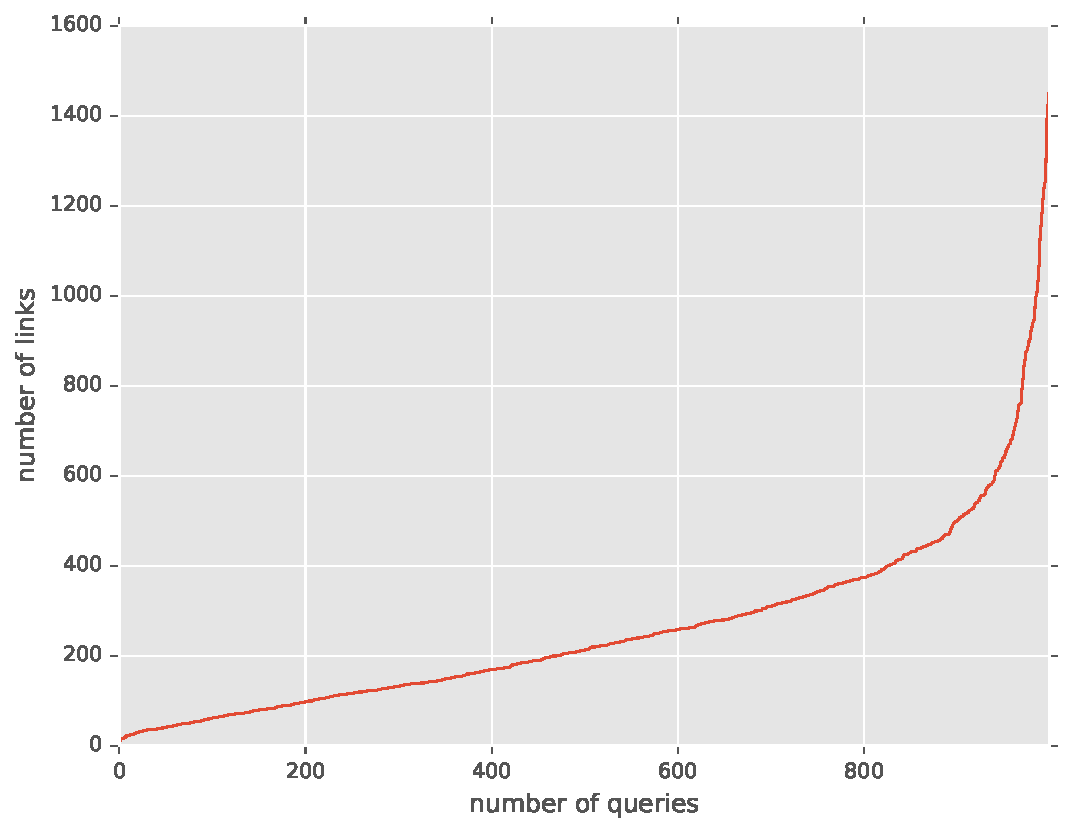
\includegraphics[width=0.95\linewidth]{images/limits_of_precision}
  \end{figure}
\end{frame}

\begin{frame}
  \frametitle{Query sensitive precision}
  \begin{itemize}
    \item different number of links per query
    \item a precision with the relative position in percentage
  \end{itemize}
  \begin{exampleblock}{Example}
    \begin{description}
      \item[links] $l_1$, $l_2$, $l_3$, $l_4$, $l_5$
      \item[labels] $y_1=5$, $y_2=4$, $y_3=3$, $y_4=2$, $y_5=1$\\
      \item[ranking] $l_1$, $l_5$, $l_3$, $l_4$, $l_2$
      \item[PP@50] $\frac{1}{3} (1 + 0 + 1) = 0.6667$
    \end{description}
  \end{exampleblock}
\end{frame}

\begin{frame}
  \frametitle{Limitations of query sensitive precision}
  \begin{figure}[tbph]
    \centering
    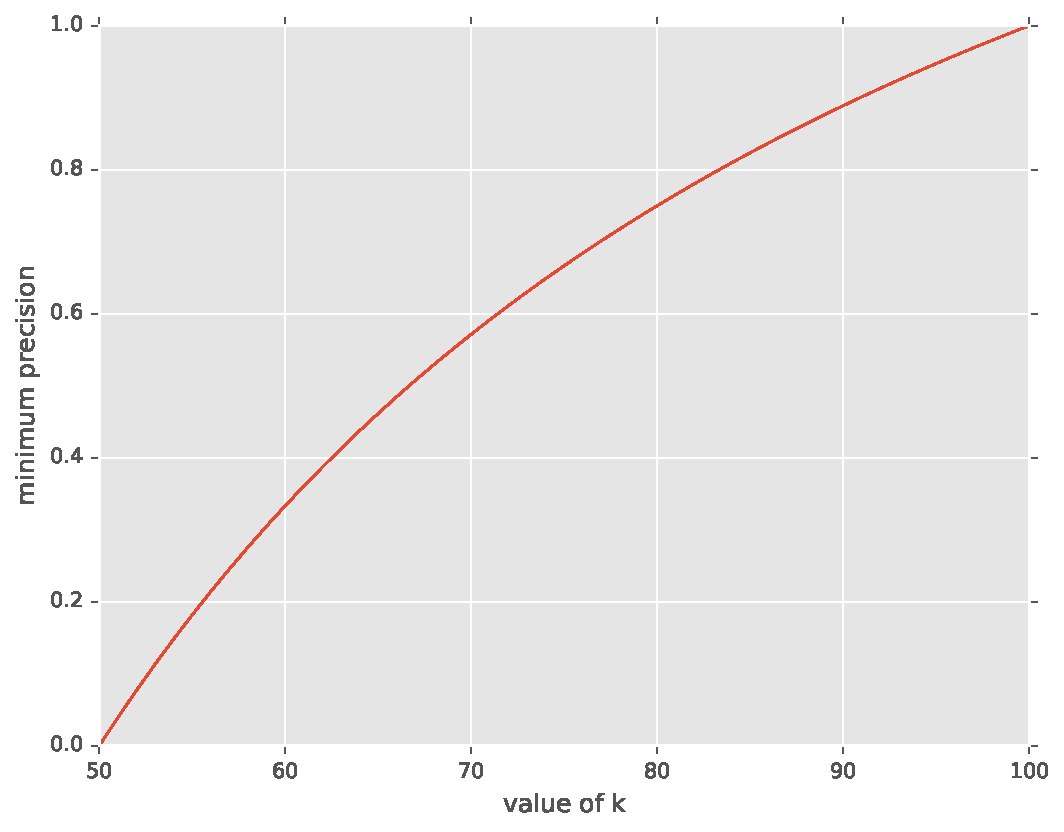
\includegraphics[width=0.95\linewidth]{images/limits_of_percentage_precision_new}
  \end{figure}
\end{frame}